\textbf{See the instruction for questions \inteval{\value{question}+1} to \inteval{\value{question}+2}.}

\begin{figure}[H]
    \centering
    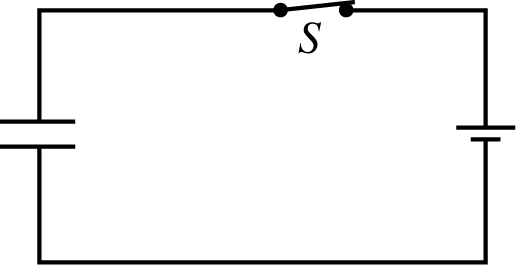
\includegraphics[scale=0.3]{images/img-007-011.png}
\end{figure}

A parallel-plate capacitor connected to a battery is fully charged with the switch $S$ closed, as shown in the circuit above. A slab of dielectric constant $\kappa>1$ is slowly inserted between the plates of the capacitor.

% Multiple Choice Question 11
\begin{questions}\setcounter{question}{10}\question
If the switch remains closed when the slab is inserted, what changes, if any, occur?

\tabto{0.75cm} Potential Difference
\tabto{5.00cm} Charge on \\
\tabto{0.75cm} \underline{Across the Plates}
\tabto{5.00cm} \underline{Positive Plate}

\begin{choices}
\choice Remains the same \tabto{4.25cm} Increases
\choice Remains the same \tabto{4.25cm} Decreases
\choice Increases        \tabto{4.25cm} Remains the same
\choice Decreases        \tabto{4.25cm} Increases
\choice Decreases        \tabto{4.25cm} Remains the same
\end{choices}\end{questions}

% Multiple Choice Question 12
\begin{questions}\setcounter{question}{11}\question
If, instead, the switch is open with the capacitor still fully charged when the slab is inserted, what changes, if any, occur?

\tabto{0.75cm} Potential Difference
\tabto{5.00cm} Charge on \\
\tabto{0.75cm} \underline{Across the Plates}
\tabto{5.00cm} \underline{Positive Plate}

\begin{choices}
\choice Remains the same \tabto{4.25cm} Increases
\choice Remains the same \tabto{4.25cm} Decreases
\choice Increases        \tabto{4.25cm} Remains the same
\choice Decreases        \tabto{4.25cm} Increases
\choice Decreases        \tabto{4.25cm} Remains the same
\end{choices}\end{questions}
